\documentclass[svgnames,11pt]{beamer}
\input{/home/tof/Documents/Cozy/latex-include/preambule_commun.tex}
\input{/home/tof/Documents/Cozy/latex-include/preambule_beamer.tex}
%\usepackage{pgfpages} \setbeameroption{show notes on second screen=left}
\author[]{Christophe Viroulaud}
\title{Arbre binaire\\Notation polonaise}
\date{\framebox{\textbf{Algo 06}}}
%\logo{}
\institute{Terminale - NSI}

\begin{document}
\begin{frame}
    \titlepage
\end{frame}
\begin{frame}
    \frametitle{}
    En 1920 le mathématicien Jan Łukasiewicz présente la \emph{notation polonaise} qui permet d'exprimer des expressions mathématiques sans utiliser de parenthèse, mais traitant néanmoins toute formule sans ambiguïté.\\
    L'expression arithmétique
    $$2~×~(3+4)$$
    devient en notation polonaise
    $$×~2+3~4$$


\end{frame}
\begin{frame}
    \frametitle{}

    Dans les années 50, Charles L. Hamblin s'intéresse à variante \emph{inversée} de cette notation. Elle est en effet particulièrement bien adaptée à la manière dont les processeurs traitent leurs opérandes.
    En notation polonaise inversée, l'expression précédente s'écrit
    $$2~3~4~+~×$$
    \note{En 1972 Hewlett-Packard sort une calculatrice financière en notation polonaise inversée = gain de temps car moins de touches à utiliser}
\end{frame}
\begin{frame}
    \frametitle{}

    \begin{framed}
        Déterminer une structure de données adaptée au calcul en notation polonaise inversée.
    \end{framed}

\end{frame}
\section{Arbre binaire}
\subsection{Définition}
\begin{frame}
    \frametitle{Arbre binaire - définition}
    \begin{aretenir}[]
        Un \textbf{arbre binaire} est une structure arborescente où chaque nœud possède \textbf{au plus} deux fils. L'ordre des nœuds-fils est pris en compte: on parle alors de fils \emph{gauche} et fils \emph{droit}.
    \end{aretenir}
    \begin{center}
        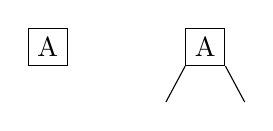
\begin{tikzpicture}
            \node[draw] (A) at (0,0) {A};
            \node[draw] (B) at (2,0) {A};

            \draw (B.south west) -- (1.5,-0.7);
            \draw (B.south east) -- (2.5,-0.7);
        \end{tikzpicture}
        \captionof{figure}{Représentations d'un nœud}
        \label{noeud}
    \end{center}

\end{frame}
\begin{frame}
    \frametitle{}

    \begin{center}
        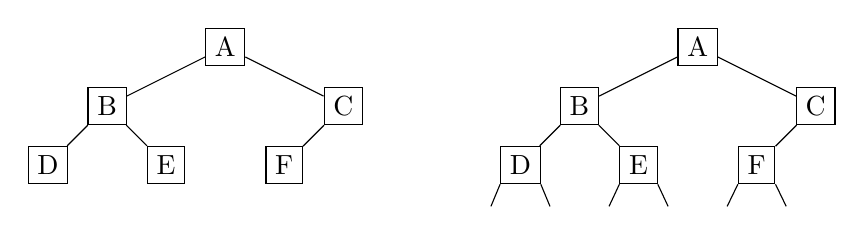
\begin{tikzpicture}[scale=0.75]
            \node[draw] (A) at (-3,0) {A};
            \node[draw] (B) at (-5,-1) {B};
            \node[draw] (C) at (-1,-1) {C};
            \node[draw] (D) at (-6,-2) {D};
            \node[draw] (E) at (-4,-2) {E};
            \node[draw] (F) at (-2,-2) {F};

            \draw (A) -- (B);
            \draw (A) -- (C);
            \draw (B) -- (D);
            \draw (B) -- (E);
            \draw (C) -- (F);

            \node[draw] (A1) at (5,0) {A};
            \node[draw] (B1) at (3,-1) {B};
            \node[draw] (C1) at (7,-1) {C};
            \node[draw] (D1) at (2,-2) {D};
            \node[draw] (E1) at (4,-2) {E};
            \node[draw] (F1) at (6,-2) {F};

            \draw (A1) -- (B1);
            \draw (A1) -- (C1);
            \draw (B1) -- (D1);
            \draw (B1) -- (E1);
            \draw (C1) -- (F1);
            \draw (D1.south west) -- (1.5,-2.7);
            \draw (D1.south east) -- (2.5,-2.7);
            \draw (E1.south west) -- (3.5,-2.7);
            \draw (E1.south east) -- (4.5,-2.7);
            \draw (F1.south west) -- (5.5,-2.7);
            \draw (F1.south east) -- (6.5,-2.7);
        \end{tikzpicture}
        \captionof{figure}{Représentations d'un arbre binaire}
        \label{arbre}
    \end{center}

\end{frame}
\subsection{vocabulaire}
\begin{frame}
    \frametitle{vocabulaire}

    \begin{aretenir}[]
        Un arbre binaire est \textbf{complet} si tous les niveaux sont remplis sauf éventuellement le dernier; les feuilles sont alors \emph{tassées à gauche}
    \end{aretenir}
    \begin{center}
        \begin{tikzpicture}
            \node[draw] (A) at (0,0) {A};
            \node[draw] (B) at (-3,-1) {B};
            \node[draw] (C) at (-5,-2) {C};
            \node[draw] (D) at (-1,-2) {D};
            \node[draw] (E) at (-6,-3) {E};
            \node[draw] (F) at (-4,-3) {F};
            \node[draw] (H) at (-2,-3) {H};
            \node[draw] (I) at (3,-1) {I};
            \node[draw] (J) at (2,-2) {J};
            \node[draw] (K) at (4,-2) {K};
            \node[draw] (L) at (0,-3) {L};
            \draw (A) -- (B);
            \draw (C) -- (B);
            \draw (C) -- (E);
            \draw (C) -- (F);
            \draw (D) -- (B);
            \draw (D) -- (H);
            \draw (A) -- (I);
            \draw (J) -- (I);
            \draw (I) -- (K);
            \draw (L) -- (D);
        \end{tikzpicture}
        \captionof{figure}{Un arbre binaire complet}
        \label{arbre}
    \end{center}
\end{frame}
\begin{frame}
    \frametitle{}

    \begin{aretenir}[]
        Un arbre binaire est \textbf{équilibré} si pour chaque nœud interne, les \emph{sous-arbres gauche et droite} ont une hauteur qui diffère au plus de 1.
    \end{aretenir}
    \begin{center}
        \begin{tikzpicture}
            \node[draw] (A) at (0,0) {A};
            \node[draw] (B) at (-3,-1) {B};
            \node[draw] (C) at (-5,-2) {C};
            \node[draw] (D) at (-1,-2) {D};
            \node[draw] (E) at (-6,-3) {E};
            \node[draw] (F) at (-4,-3) {F};
            \node[draw] (H) at (-2,-3) {H};
            \node[draw] (I) at (3,-1) {I};
            \node[draw] (J) at (2,-2) {J};
            \node[draw] (K) at (4,-2) {K};
            \node[draw] (L) at (5,-3) {L};
            \draw (A) -- (B);
            \draw (C) -- (B);
            \draw (C) -- (E);
            \draw (C) -- (F);
            \draw (D) -- (B);
            \draw (D) -- (H);
            \draw (A) -- (I);
            \draw (J) -- (I);
            \draw (I) -- (K);
            \draw (L) -- (K);
        \end{tikzpicture}
        \captionof{figure}{Un arbre binaire équilibré non complet}
        \label{arbre}
    \end{center}
\end{frame}
\begin{frame}
    \frametitle{}

    \begin{aretenir}[]
        Un arbre binaire est \textbf{parfait} si tous les niveaux sont remplis.
    \end{aretenir}
    \begin{center}
        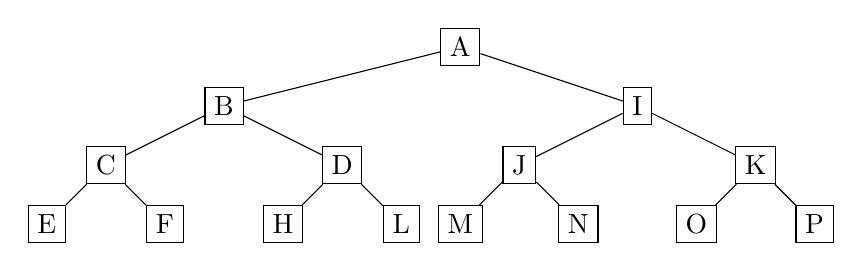
\begin{tikzpicture}[scale=0.75]
            \node[draw] (A) at (1,0) {A};
            \node[draw] (B) at (-3,-1) {B};
            \node[draw] (C) at (-5,-2) {C};
            \node[draw] (D) at (-1,-2) {D};
            \node[draw] (E) at (-6,-3) {E};
            \node[draw] (F) at (-4,-3) {F};
            \node[draw] (H) at (-2,-3) {H};
            \node[draw] (I) at (4,-1) {I};
            \node[draw] (J) at (2,-2) {J};
            \node[draw] (K) at (6,-2) {K};
            \node[draw] (L) at (0,-3) {L};
            \node[draw] (M) at (1,-3) {M};
            \node[draw] (N) at (3,-3) {N};
            \node[draw] (O) at (5,-3) {O};
            \node[draw] (P) at (7,-3) {P};

            \draw (A) -- (B);
            \draw (C) -- (B);
            \draw (C) -- (E);
            \draw (C) -- (F);
            \draw (D) -- (B);
            \draw (D) -- (H);
            \draw (A) -- (I);
            \draw (J) -- (I);
            \draw (I) -- (K);
            \draw (L) -- (D);
            \draw (J) -- (M);
            \draw (J) -- (N);
            \draw (K) -- (O);
            \draw (K) -- (P);
        \end{tikzpicture}
        \captionof{figure}{Un arbre binaire parfait}
        \label{arbre}
    \end{center}
\end{frame}

\subsection{Propriétés}
\begin{frame}
    \frametitle{Propriétés}
    \begin{aretenir}[]
        Dans un arbre binaire, la taille \emph{N} et la hauteur \emph{h} sont liées par les inégalités:
        \begin{center}
            $h+1 \leqslant N \leqslant 2^{h+1}-1$
        \end{center}
    \end{aretenir}
    \begin{center}
        \begin{tikzpicture}
            \node[draw] (A) at (0,0) {A};
            \node[draw] (B) at (-3,-1) {B};
            \node[draw] (C) at (-5,-2) {C};
            \node[draw] (D) at (-1,-2) {D};
            \node[draw] (E) at (-6,-3) {E};
            \node[draw] (F) at (-4,-3) {F};
            \node[draw] (H) at (-2,-3) {H};
            \node[draw] (I) at (3,-1) {I};
            \node[draw] (J) at (2,-2) {J};
            \node[draw] (K) at (4,-2) {K};
            \node[draw] (L) at (0,-3) {L};
            \draw (A) -- (B);
            \draw (C) -- (B);
            \draw (C) -- (E);
            \draw (C) -- (F);
            \draw (D) -- (B);
            \draw (D) -- (H);
            \draw (A) -- (I);
            \draw (J) -- (I);
            \draw (I) -- (K);
            \draw (L) -- (D);
        \end{tikzpicture}
        \captionof{figure}{Un arbre binaire complet}
        \label{arbre}
    \end{center}

\end{frame}
\begin{frame}
    \frametitle{Démonstration}

    \begin{center}
        \begin{tikzpicture}
            \node[draw] (A) at (0,0) {A};
            \node[draw] (B) at (-1,-1) {B};
            \node[draw] (C) at (-2,-2) {C};
            \node[draw] (D) at (-3,-3) {D};

            \draw (A) -- (B);
            \draw (C) -- (B);
            \draw (C) -- (D);
        \end{tikzpicture}
        \captionof{figure}{Un arbre binaire minimal}
        \label{arbre}
    \end{center}
    $$h+1 \leqslant N$$
\end{frame}
\begin{frame}
    \frametitle{}

    \begin{center}
        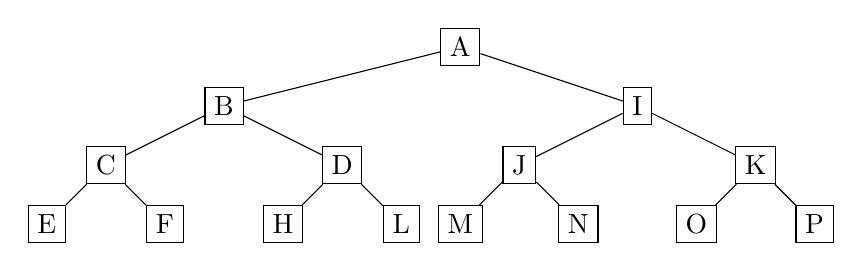
\begin{tikzpicture}[scale=0.75]
            \node[draw] (A) at (1,0) {A};
            \node[draw] (B) at (-3,-1) {B};
            \node[draw] (C) at (-5,-2) {C};
            \node[draw] (D) at (-1,-2) {D};
            \node[draw] (E) at (-6,-3) {E};
            \node[draw] (F) at (-4,-3) {F};
            \node[draw] (H) at (-2,-3) {H};
            \node[draw] (I) at (4,-1) {I};
            \node[draw] (J) at (2,-2) {J};
            \node[draw] (K) at (6,-2) {K};
            \node[draw] (L) at (0,-3) {L};
            \node[draw] (M) at (1,-3) {M};
            \node[draw] (N) at (3,-3) {N};
            \node[draw] (O) at (5,-3) {O};
            \node[draw] (P) at (7,-3) {P};

            \draw (A) -- (B);
            \draw (C) -- (B);
            \draw (C) -- (E);
            \draw (C) -- (F);
            \draw (D) -- (B);
            \draw (D) -- (H);
            \draw (A) -- (I);
            \draw (J) -- (I);
            \draw (I) -- (K);
            \draw (L) -- (D);
            \draw (J) -- (M);
            \draw (J) -- (N);
            \draw (K) -- (O);
            \draw (K) -- (P);
        \end{tikzpicture}
        \captionof{figure}{Un arbre binaire parfait}
        \label{arbre}
    \end{center}

    \begin{itemize}
        \item niveau 0: $2^0=1$ nœuds
        \item niveau 1: $2^1=2$ nœuds
        \item \dots
        \item niveau h: $2^h$ nœuds
    \end{itemize}
    \begin{center}
        On double le nombre de nœuds à chaque niveau.

    \end{center}

\end{frame}
\begin{frame}
    \frametitle{}

    Somme des premiers termes d'une suite géométrique: $$\sum_{k=0}^{h}{2^k}=u_0×\dfrac{1-q^{h+1}}{1-q}$$
    $$\sum_{k=0}^{h}{2^k}=1×\dfrac{1-2^{h+1}}{1-2}$$
    $$\sum_{k=0}^{h}{2^k}=2^{h+1}-1$$

    \begin{center}
        La taille maximale est inférieure ou égale à $2^{h+1}-1$
    \end{center}
\end{frame}
\begin{frame}
    \frametitle{}

    \begin{aretenir}[]
        L'inégalité est vérifiée:
        $$h+1 \leqslant N \leqslant 2^{h+1}-1$$
    \end{aretenir}
    \begin{aretenir}[Remarque]


        Si on définit la hauteur comme le nombre de nœuds maximum entre la racine et une feuille, on a: $$h \leqslant N \leqslant 2^{h}-1$$

    \end{aretenir}
\end{frame}
\section{Représentation d'une expression mathématique}
\subsection{Arbre binaire}
\begin{frame}
    \frametitle{Représentation d'une expression mathématique}

    Une expression mathématique applique une \emph{opération} sur deux \emph{opérandes}. Un arbre binaire permet donc de représenter n'importe quelle opération.
    \begin{center}
        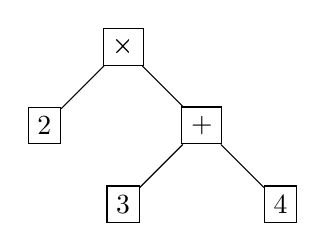
\begin{tikzpicture}
            \node[draw] (x) at (0,0) {×};
            \node[draw] (2) at (-1,-1) {2};
            \node[draw] (plus) at (1,-1) {+};
            \node[draw] (3) at (0,-2) {3};
            \node[draw] (4) at (2,-2) {4};

            \draw (x) -- (2);
            \draw (x) -- (plus);
            \draw (plus) -- (3);
            \draw (plus) -- (4);

        \end{tikzpicture}
        \captionof{figure}{$2~×~(3+4)$}
        \label{arbre}
    \end{center}

\end{frame}
\subsection{Représentation en Python}
\begin{frame}[fragile]
    \frametitle{Représentation en Python}

    \begin{center}
        \begin{lstlisting}[language=Python , basicstyle=\ttfamily\small, xleftmargin=1em, xrightmargin=1em]
class Noeud:

def __init__(self, v, g, d):
    self.valeur = v
    self.gauche = g
    self.droite = d
\end{lstlisting}
        \captionof{code}{Représentation d'un nœud}
        \label{CODE}
    \end{center}

\end{frame}
\begin{frame}
    \frametitle{}
    \begin{center}
        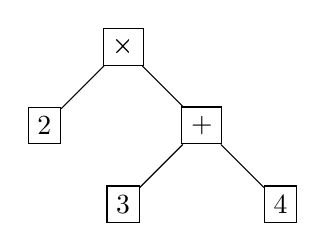
\begin{tikzpicture}
            \node[draw] (x) at (0,0) {×};
            \node[draw] (2) at (-1,-1) {2};
            \node[draw] (plus) at (1,-1) {+};
            \node[draw] (3) at (0,-2) {3};
            \node[draw] (4) at (2,-2) {4};

            \draw (x) -- (2);
            \draw (x) -- (plus);
            \draw (plus) -- (3);
            \draw (plus) -- (4);

        \end{tikzpicture}
        \captionof{figure}{$2~×~(3+4)$}
        \label{calcul}
    \end{center}
\begin{activite}
En utilisant la classe \textbf{\texttt{Noeud}} écrire la variable \textbf{\texttt{arbre}} qui représente l'expression \ref{calcul}.
\end{activite}

\end{frame}
\begin{frame}[fragile]
    \frametitle{Correction}

\begin{center}
\begin{lstlisting}[language=Python , basicstyle=\ttfamily\small, xleftmargin=1em, xrightmargin=0em]
arbre = Noeud("×",
                Noeud(2, None, None),
                Noeud("+",
                        Noeud(3, None, None),
                        Noeud(4, None, None)))
\end{lstlisting}
\end{center}    

\end{frame}
\begin{frame}
    \frametitle{}

Pour calculer la taille d'un arbre, il faut:
\begin{itemize}
    \item calculer récursivement la taille du fils gauche,
    \item calculer récursivement la taille du fils droit,
    \item ajouter 1 (pour le nœud en cours).
\end{itemize}
\begin{activite}
\begin{enumerate}
    \item Dans l'algorithme de calcul de la taille, quel est le cas limite?
    \item Écrire la fonction récursive \textbf{\texttt{taille(a: Noeud) $\rightarrow$ int}} qui renvoie la taille de l'arbre.
\end{enumerate}
\end{activite}
\end{frame}
\begin{frame}[fragile]
    \frametitle{Correction}

\begin{center}
\begin{lstlisting}[language=Python , basicstyle=\ttfamily\small, xleftmargin=.5em, xrightmargin=-1em]
def taille(a: Noeud) -> int:
    """
    renvoie le nombre de noeuds de l'arbre a
    """
    if a is None:
        return 0
    else:
        return 1 + taille(a.gauche) + taille(a.droite)
\end{lstlisting}
\captionof{code}{Taille de l'arbre}
\label{CODE}
\end{center}    

\end{frame}
\begin{frame}
    \frametitle{}

\begin{activite}
\begin{enumerate}
    \item Écrire la fonction récursive \textbf{\texttt{hauteur(a: Noeud) $\rightarrow$ int}} qui renvoie la hauteur de l'arbre binaire. On utilisera la fonction Python \textbf{\texttt{max}} pour comparer la taille des fils gauche et droit.
    \item Étudier la complexité des fonctions \textbf{\texttt{taille}} et \textbf{\texttt{hauteur}}.
\end{enumerate}
\end{activite}

\end{frame}
\begin{frame}[fragile]
    \frametitle{Correction}

\begin{center}
\begin{lstlisting}[language=Python , basicstyle=\ttfamily\small, xleftmargin=.2em, xrightmargin=-4em]
def hauteur(a: Noeud) -> int:
    """
    hauteur max de l'arbre a
    """
    if a is None:
        return 0
    else:
        return 1 + max(hauteur(a.gauche), hauteur(a.droite))
\end{lstlisting}
\captionof{code}{Hauteur de l'arbre}
\label{CODE}
\end{center}   

\end{frame}
\begin{frame}
    \frametitle{}

    Dans les deux fonctions on parcourt une et une seule fois chaque nœud. La complexité est \textbf{linéaire}.

\end{frame}
\subsection{Parcours en profondeur}
\begin{frame}
    \frametitle{Parcours en profondeur}

    \begin{center}
        Dans un arbre binaire, on commence par parcourir le sous-arbre gauche avant celui de droite.
    \end{center}

\end{frame}
\begin{frame}[fragile]
    \frametitle{}

\begin{itemize}
\item<1-> \textbf{Parcours préfixe:}
\begin{lstlisting}[language=Python , basicstyle=\ttfamily\small, xleftmargin=.2em, xrightmargin=0em]
parcours préfixe(arbre)
    affiche(valeur)
    parcours préfixe(sous-arbre gauche)
    parcours préfixe(sous-arbre droit)
\end{lstlisting}
\item<2-> \textbf{Parcours infixe:}
\begin{lstlisting}[language=Python , basicstyle=\ttfamily\small, xleftmargin=.2em, xrightmargin=0em]
parcours infixe(arbre)
    parcours infixe(sous-arbre gauche)
    affiche(valeur)
    parcours infixe(sous-arbre droit)
\end{lstlisting}
\item<3-> \textbf{Parcours postfixe (ou suffixe):}
\begin{lstlisting}[language=Python , basicstyle=\ttfamily\small, xleftmargin=.2em, xrightmargin=0em]
parcours postfixe(arbre)
    parcours postfixe(sous-arbre gauche)
    parcours postfixe(sous-arbre droit)
    affiche(valeur)
\end{lstlisting}
\end{itemize}

\end{frame}
\begin{frame}
    \frametitle{}

    \begin{activite}
        \begin{enumerate}
        \item Écrire les trois fonctions \emph{récursives} de parcours qui affichent (\textbf{\texttt{print}}) directement la valeur du nœud traversé.
        \item Adapter ces fonctions pour renvoyer un tableau ordonné des nœuds traversés.
        \item Quel parcours implémente la notation polonaise inverse?
        \item Étudier la complexité des fonctions de parcours.
        \end{enumerate}
        \end{activite}

\end{frame}
\begin{frame}[fragile]
    \frametitle{Correction}

\begin{center}
\begin{lstlisting}[language=Python , basicstyle=\ttfamily\small, xleftmargin=1em, xrightmargin=1em]
def prefixe(a: Noeud) -> None:
    if a is not None:
        print(a.valeur, end=" ")
        prefixe(a.gauche)
        prefixe(a.droite)
\end{lstlisting}
\end{center}    
\begin{lstlisting}[language=Python , basicstyle=\ttfamily\small, xleftmargin=1em, xrightmargin=1em]
prefixe(arbre)
\end{lstlisting}
\begin{lstlisting}[language=Python , basicstyle=\ttfamily\small, xleftmargin=1em, xrightmargin=1em]
'×' 2 '+' 3 4
\end{lstlisting}
\end{frame}
\begin{frame}[fragile]
    \frametitle{Correction}

\begin{center}
\begin{lstlisting}[language=Python , basicstyle=\ttfamily\small, xleftmargin=1em, xrightmargin=1em]
def infixe(a: Noeud) -> None:
    if a is not None:
        infixe(a.gauche)
        print(a.valeur, end=" ")
        infixe(a.droite)


def postfixe(a: Noeud) -> None:
    if a is not None:
        postfixe(a.gauche)
        postfixe(a.droite)
        print(a.valeur, end=" ")
\end{lstlisting}
\end{center}    

\end{frame}
\begin{frame}[fragile]
    \frametitle{}

\begin{center}
\begin{lstlisting}[language=Python , basicstyle=\ttfamily\small, xleftmargin=.5em, xrightmargin=0em]
def prefixe_tab(a: Noeud, parcours: list) -> None:
    if a is not None:
        parcours.append(a.valeur)
        prefixe_tab(a.gauche, parcours)
        prefixe_tab(a.droite, parcours)
\end{lstlisting}
\end{center}
\begin{aretenir}[Remarque]
Le tableau passé en paramètre est une \textbf{référence} à un tableau du programme principal
\end{aretenir}
\begin{center}
\begin{lstlisting}[language=Python , basicstyle=\ttfamily\small, xleftmargin=2em, xrightmargin=2em]
tab_prefixe = []
prefixe_tab(arbre, tab_prefixe)
print("préfixe ", tab_prefixe)
\end{lstlisting}
\captionof{code}{Appel}
\label{CODE}
\end{center}
\end{frame}
\begin{frame}[fragile]
    \frametitle{}

\begin{center}
\begin{lstlisting}[language=Python , basicstyle=\ttfamily\small, xleftmargin=.5em, xrightmargin=0em]
def infixe_tab(a: Noeud, parcours: list) -> None:
    if a is not None:
        infixe_tab(a.gauche, parcours)        
        parcours.append(a.valeur)
        infixe_tab(a.droite, parcours)



def postfixe_tab(a: Noeud, parcours: list) -> None:
    if a is not None:
        postfixe_tab(a.gauche, parcours)        
        postfixe_tab(a.droite, parcours)
        parcours.append(a.valeur)
\end{lstlisting}
\end{center}

\end{frame}
\begin{frame}[fragile]
    \frametitle{}

\begin{center}
\begin{lstlisting}[language=Python , basicstyle=\ttfamily\small, xleftmargin=1em, xrightmargin=1em]
# notation polonaise
préfixe  ['×', 2, '+', 3, 4]

# notation usuelle
infixe  [2, '×', 3, '+', 4]

# notation polonaise inverse
postfixe  [2, 3, 4, '+', '×']
\end{lstlisting}
\end{center}
\begin{aretenir}[Remarque]
Dans la notation usuelle les parenthèses sont obligatoires pour éviter les ambiguïtés.
\end{aretenir}
\end{frame}
\begin{frame}[fragile]
    \frametitle{}

\begin{center}
\begin{lstlisting}[language=Python , basicstyle=\ttfamily\small, xleftmargin=2em, xrightmargin=2em]
def prefixe_tab2(a: Noeud) -> list:
    if a is not None:
        # concatène les tableaux construits
        return [a.valeur] + \
                prefixe_tab2(a.gauche) + \
                prefixe_tab2(a.droite)
    else:
        return []
\end{lstlisting}
\captionof{code}{Version avec concaténation}
\label{CODE}
\end{center}    
\begin{aretenir}[Remarque]
En fin de parcours, il faut renvoyer un tableau vide pour concaténer des structures de même type.
\end{aretenir}
\end{frame}
\begin{frame}
    \frametitle{}

    \begin{aretenir}[]
Un parcours en profondeur (ou en largeur) visite une et une seule fois chaque nœud. La complexité en temps est \textbf{linéaire}.
    \end{aretenir}

\end{frame}
\end{document}